\subsection{Model parameter estimates in the limit of large data sets} \label{sec:largedata}

The individual \MAP{}s in BR13 contained typically between 100 and 800 objects, so that each \MAP{} implied a quite broad \pdf{} for the model parameters $\pmodel{}$. Here we explore what happens in the limit of much larger samples, say $N_{*} = 20,000$ objects.  As outlined in Section \ref{sec:likelihood}, the immediate consequence of larger samples is given by the likelihood normalization requirement $\log(1+\delta M_\text{tot})\le 1/N_{*}$ (Equation \ref{eq:accuracycondition}), which is the modelling aspect that drives the computing time. This issues aside, we would however expect that in the limit of large data sets with vanishing measurement uncertainties the \pdf{}s of the \pmodel{} become Gaussian, with a \pdf{} width (i.e., the standard error (SE) on the parameter estimate) that scales as $1/\sqrt{N_{*}}$. Further, we must verify that any bias in the \pdf{} expectation value is considerably less than the error, even for quite large samples.

%====================================================================

%FIGURE: width of likelihood propto 1/sqrt(N)

\begin{figure}[!htbp]
\plotone{figs/sqrtNiso_Stddev_Vs_N.eps}
\caption{The width of the \pdf{} (see Equation \ref{eq:prob}) for two fit parameters found from analyses of 132 mock data sets vs. the number of stars in each data set, $N_{*}$. (The mock data was created according to the model parameters given in Test \ref{test:sqrtNiso} in Table \ref{tbl:tests}.) The relative standard error (SE) was found from a Gaussian fit to the marginalized \pdf{} for each model parameter. As can be seen, for large data samples the width of the \pdf{} scales with $1/\sqrt{N_{*}}$ as expected.} 
\label{fig:sqrtNiso}
\end{figure}

%====================================================================

%====================================================================

%FIGURE: central limit theorem is satisfied

\begin{figure}[!htbp]
\centering
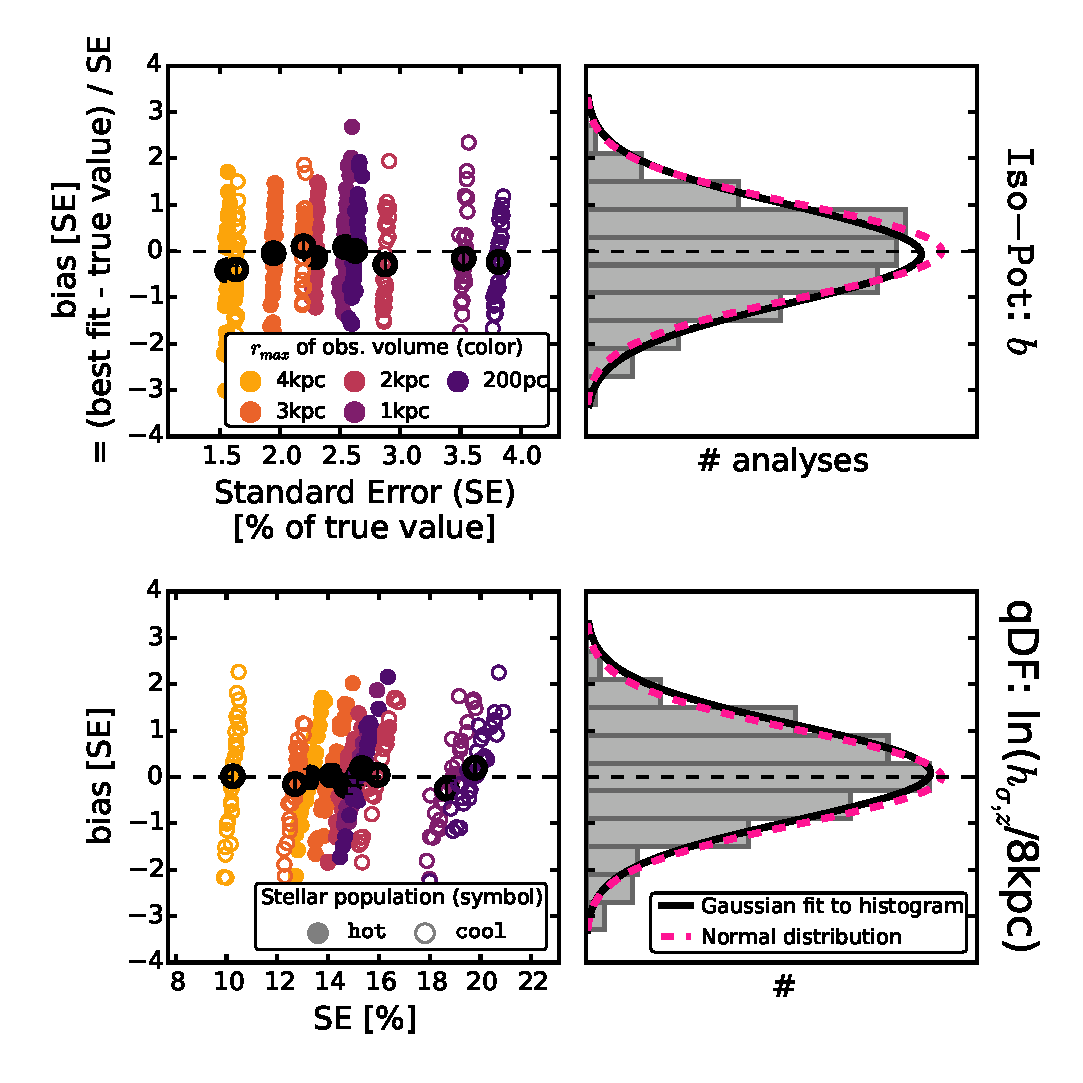
\includegraphics[width=\columnwidth]{figs/isoSph_CLT_2.eps}
\caption{(Un-)bias of the parameter estimates. Maximum likelihood estimators converge to the true parameter values for large numbers of data points and have a Gaussian spread---if the model assumptions are fulfilled. To test that these conditions are satisfied for \RM{}, we create 320 mock data sets, which come from two different stellar populations and five spherical observation volumes (see legends). (All model parameters are summarized in Table \ref{tbl:tests} as Test \ref{test:isoSph_CLT}.) Bias and relative standard error (SE) are derived from the marginalized \pdf{} for two model parameters (isochrone scale length $b$ in the first row and qDF parameter $h_{\sigma,z}$ in the second row). The second column displays a histogram of the 320 bias offsets. As it closely follows a Normal distribution, our modelling method is therefore well-behaved and unbiased. The black dots denote the \pdf{} expectation value for the 32 analyses belonging to the same $\pmodel{}$.}
\label{fig:isoSph_CLT}
\end{figure}

%====================================================================

%====================================================================

%FIGURE: Does shape and position of obs. volume matter?


\begin{figure}[!htbp]
\centering
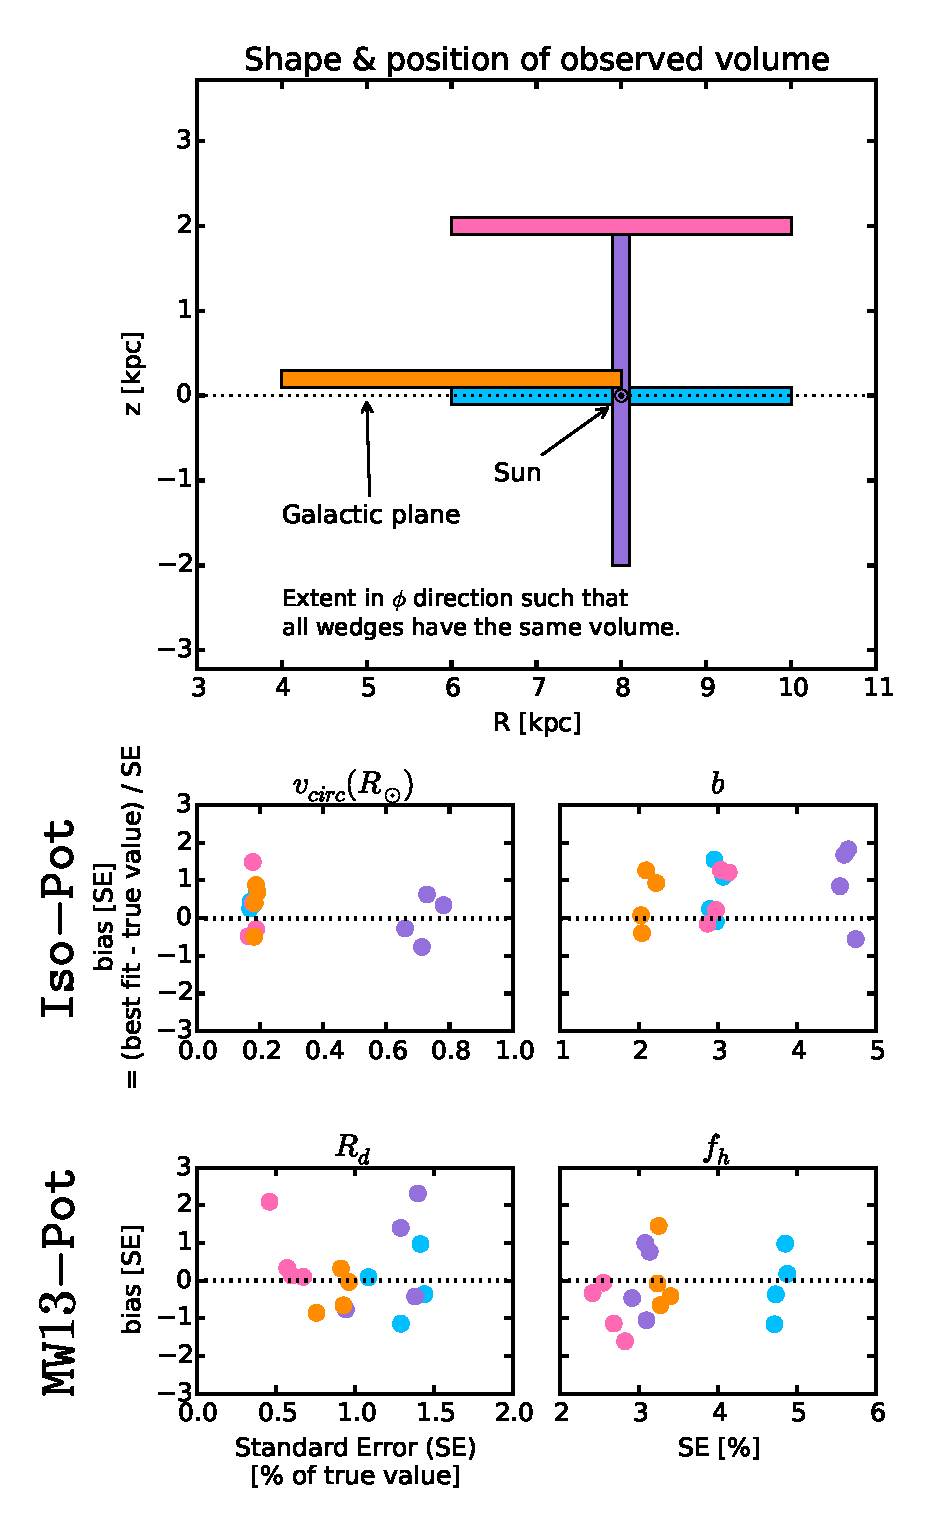
\includegraphics[width=\columnwidth]{figs/wedFlexVol_bias_vs_SE.eps}
\caption{Bias vs. standard error in recovering the potential parameters for mock data sets drawn from four different wedge-shaped test observation volumes within the Galaxy (illustrated in the upper panel; the corresponding analyses are colour-coded) and two different potentials (\texttt{Iso-Pot} and \texttt{MW13-Pot} from Table \ref{tbl:referencepotentials}; see also Test \ref{test:wedFlexVol} in Table \ref{tbl:tests} for all model parameters used). Standard error and offset were determined from a Gaussian fit to the marginalized \pdf{}. The angular extent of each wedge-shaped observation volume was adapted such that all have a volume of $4.5~\text{kpc}^3$, even though their extent in $(R,z)$ is different. Overall there is no clear trend that an observation volume around the Sun, above the disk or at smaller Galactocentric radii should give remarkably better constraints on the potential than the other volumes.}
\label{fig:wedFlexVol_bias_vs_SE}
\end{figure}


%====================================================================

Using sets of mock data, created according to the procedure in Section \ref{sec:mockdata} and a fiducial model for \pmodel{} (see Table \ref{tbl:tests}, Tests \ref{test:sqrtNiso}, \ref{test:isoSph_CLT}, and \ref{test:isoSphFlex}), we verified that \RM{} satisfies all these conditions and expectations: Figure \ref{fig:isoSphFlex_triangleplot} illustrates the joint \pdf{}s of all \pmodel{}. The \pdf{} is a multivariate Gaussian that projects into Gaussians when considering the marginalized \pdf{} for all the individual \pmodel{}. Figure \ref{fig:sqrtNiso} then demonstrates that the \pdf{} width indeed scales as $1/\sqrt{N_{*}}$. Figure \ref{fig:isoSph_CLT} illustrates even more that \RM{} behaves like an unbiased maximum likelihood estimator: The average parameter estimates from many mock samples with identical underlying \pmodel{} are very close to the input \pmodel{}, and the distribution of the actual parameter estimates are a Gaussian around it. 